% Activate the following line by filling in the right side. If for example the name of the root file is Main.tex, write
% "...root = Main.tex" if the chapter file is in the same directory, and "...root = ../Main.tex" if the chapter is in a subdirectory.
 
%!TEX root =  

\chapter{Documentation}\label{doc}

\minitoc

This section provides documentation for the Privacy Advisor system. It gives an overview over the available documentation of source code, instructions for how to compile and install the system, and how it is used via. its GUI and command line interfaces.

\section{Source Code Documentation}

The source code is documented using JavaDoc which is 	a tool that generates documentation in HTML format based on source code comments in Java, and is a standard part of the Java SDK. The JavaDoc for the Privacy Advisor system follows Sun Microsystems' style guide for writing JavaDoc comments\footnote{See: http://www.oracle.com/technetwork/java/javase/documentation/index-137868.html}. Source code documentation plays an important role in this project, as it is an early software prototype to be used in research which means that the code is then likely to be modified. The aim of the source code documentation is to supplement UML design documents to facilitate future development.

\section{Installation}

\subsection{Local Installation}
To make the program run outside of the Eclipse environment it have to be exported as a runnable jar file. This can be done by right clicking the project in eclipse, choose "Export", type in "jar" in the in the new windows that opened up and choose "Runnable Jar File", before clicking "next". These two steps are showed in the two figures \ref{exportFirstStep} and \ref{exportSecondStep}.

\begin{centering}
  \begin{figure}
    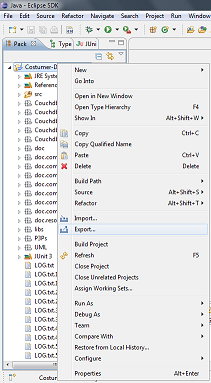
\includegraphics{Documentation/export.png}
    \caption{First step: right click and choose "export".}
    \label{exportFirstStep}
  \end{figure}
\end{centering}

\begin{centering}
  \begin{figure}
    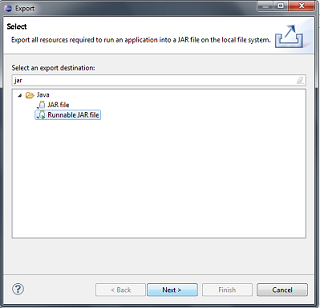
\includegraphics{Documentation/export_jar.png}
    \caption{Second step: choose runnable jar.}
    \label{exportSecondStep}
  \end{figure}
\end{centering}

Then we have to choose which classfile we want to be the main class, in the "Launch configuration" dropdown menu we can choose between the two classes PrivacyAdviser and PrivacyAdvisorGUI. The first one is choosen if we want to run the whole program froim the command line, and the second one if we want to use the GUI. Then choose the export destination, and "Package requires libraries into generated JAR" as the library handling. Pressing finish now should start exporting the program. These steps are shown in figure \ref{exportLastStep}.

\begin{centering}
  \begin{figure}
    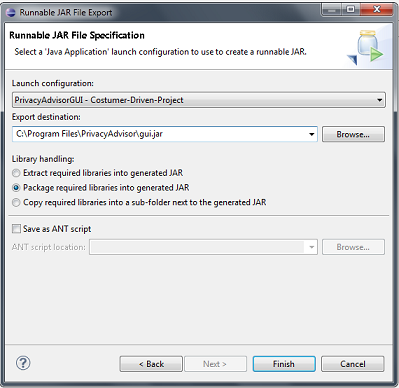
\includegraphics{Documentation/export_last.png}
    \caption{Third step: choose launch config, destination and library handling.}
    \label{exportLastStep}
  \end{figure}
\end{centering}

Before running the program we have to put the PrivacyAdviser.cfg file in the same folder as the exported jar file. To run the program, open the command prompt and locate to the folder where the jar file is stored. Then write the command java -jar filename.jar, and now the program should start (even if it's the cli or gui version). This is show in figure \ref{runProgram}.

\begin{centering}
  \begin{figure}
    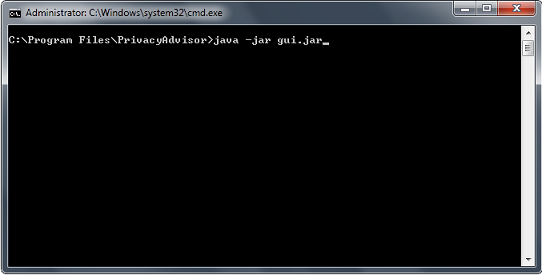
\includegraphics{Documentation/run.png}
    \caption{Run the program.}
    \label{runProgram}
  \end{figure}
\end{centering}

\subsection{Server Installation}

\section{User Interfaces}

\subsection{Graphical User Interface}

\subsection{Command Line Interface}

\subsubsection{Configuration Files}

Table~\ref{configTable} gives an overview over the configuration file parameters.

\begin{center}
  \begin{table}[h!]
    \label{configTable}
    \begin{tabular} { | l | l | p{7cm} | }
      \hline
      \textbf{Item} & \textbf{Datatype} & \textbf{Description} \\ \hline
      loglocation & string/filepath  & where the log is written to. can't be changed once the UI is  called. \\ \hline
      loglevel & string/logging level	& what level to log at. \\ \hline
      inDBLoc & string/filepath	& where to read the past history from. \\ \hline
      outDBLoc & string/filepath & where to write DB- defaults to where it reads from. \\ \hline
      inWeightsLoc& string/filepath & where to read the weights config file from. \\ \hline
      outWeightsLoc	& string/filepath & where to write DB- defaults to where it reads from. \\ \hline
      newDB & string/boolean & are we overwriting/ignoring an old database. \\ \hline
      p3pLocation & string/filepath & a p3p to be added to the history. \\ \hline
      p3pDirLocation	& string/FOLDERpath& a folder of p3ps to be added to the history. \\ \hline
      blanketAccept & string/boolean & accept the advisers recommendation. \\ \hline
      newPolicyLoc & string/filepath	& the new policy to be parsed. \\ \hline
      userInit & string/boolean	& true if some initialization occurs via the user interface. \\ \hline
      userResponse & string/action	& the response to the suggestion, if know beforehand. \\ \hline
      cbrV & string/CBR & parses for algorithms, etc to use. See CBR:parse(String). \\ \hline
      userIO & string/UIO	& the user interface to use. see Gio:selectUI. \\ \hline
      policyDB & string/policyDB & select the database type. see Gio:selectPDB . \\ \hline
      genConfig	& string/filepath & load an alternate configuration file. \\ \hline
      networkRType & string/classname & the name of a networkR class. \\ \hline
      networkROptions & string/commasepoptions	& the options necessary for the above networkR class. \\ \hline
      confidenceLevel & string/double & the confidence level at which the algorithm trusts itself; if below this, it uses the server's suggestion. \\ \hline
      useNet & string/boolean & whether to activate network functionality. \\ \hline
      \hline
    \end{tabular}
    \caption{Configuration file parameters.}
  \end{table}
\end{center}

\subsubsection{Building a Database}

\textbf{CLI}: To build a new database from a directory \texttt{P3PDir} holding P3P files, Privacy
Advisor can be called from the command line in the following fashion:
\texttt{PrivacyAdvisor -newDB  true -outDBLoc new.db
  -p3pDirLocation P3PDir}.

\textbf{GUI}: To build a new database in the similar fashion using the
graphical user interface, the configuration window can be set up
similarly to that illustrated in figure[XXXX].



\subsubsection{Loading and Viewing a Database}



\subsubsection{Parsing a P3P Policy}
